\documentclass[12pt,titlepage]{article}
\usepackage[margin=1in]{geometry}
\usepackage{fancyhdr}
\usepackage{listings}
\usepackage{amsmath}
\usepackage{graphicx}
\setlength\parindent{0pt}
\fancyhf{}
\rfoot{Page \thepage}

\begin{document}
\begin{titlepage}
	\centering
	\vfill
	{\bfseries\Large
		Joseph Morgan\\
		\large
		Homework 10\\
		\vskip2cm
		CISP440\\
	}
	\vfill
	\vfill
	\vfill
\end{titlepage}
\section{Source code for inverse table generator program}

\subsection*{inverse\_table.h}}

\lstinputlisting[
breaklines=true,
language=C++,
basicstyle=\footnotesize,
numbers=left,
numberstyle=\tiny,
tabsize=2
]{/home/joe/dev/cpp/CISP440/encryption/inverse_table.h}

\subsection*{inverse\_table.cpp}

\lstinputlisting[
breaklines=true,
language=C++,
basicstyle=\footnotesize,
numbers=left,
numberstyle=\tiny,
tabsize=2
]{/home/joe/dev/cpp/CISP440/encryption/inverse_table.cpp}
\section{Source code for decryption program}

\subsection*{decrytor.h}

\lstinputlisting[
breaklines=true,
language=C++,
basicstyle=\footnotesize,
numbers=left,
numberstyle=\tiny,
tabsize=2
]{/home/joe/dev/cpp/CISP440/encryption/decryptor.h}

\subsection*{decrytor.cpp}

\lstinputlisting[
breaklines=true,
language=C++,
basicstyle=\footnotesize,
numbers=left,
numberstyle=\tiny,
tabsize=2
]{/home/joe/dev/cpp/CISP440/encryption/decryptor.cpp}
\subsection*{main.cpp}
\lstinputlisting[
breaklines=true,
language=C++,
basicstyle=\footnotesize,
numbers=left,
numberstyle=\tiny,
tabsize=2
]{/home/joe/dev/cpp/CISP440/encryption/main.cpp}
\section{Inverse function tables printout}
\lstinputlisting[
breaklines=true,
language=C++,
basicstyle=\footnotesize,
numbers=left,
numberstyle=\tiny,
tabsize=2
]{/home/joe/dev/cpp/CISP440/encryption/output.txt}
\section{Key value}
Key value was: c
\section{Inverse function composition order}
I know you said this part was easier than it sounds, but I'm really at a loss for what
it means and at this point I've waited too long to email and ask.. My loss I guess :(
I feel like the answer to this has got to be in my code somewhere but I can't seem
to work out what exactly I should put in this section.
\section{Decrypted Output}
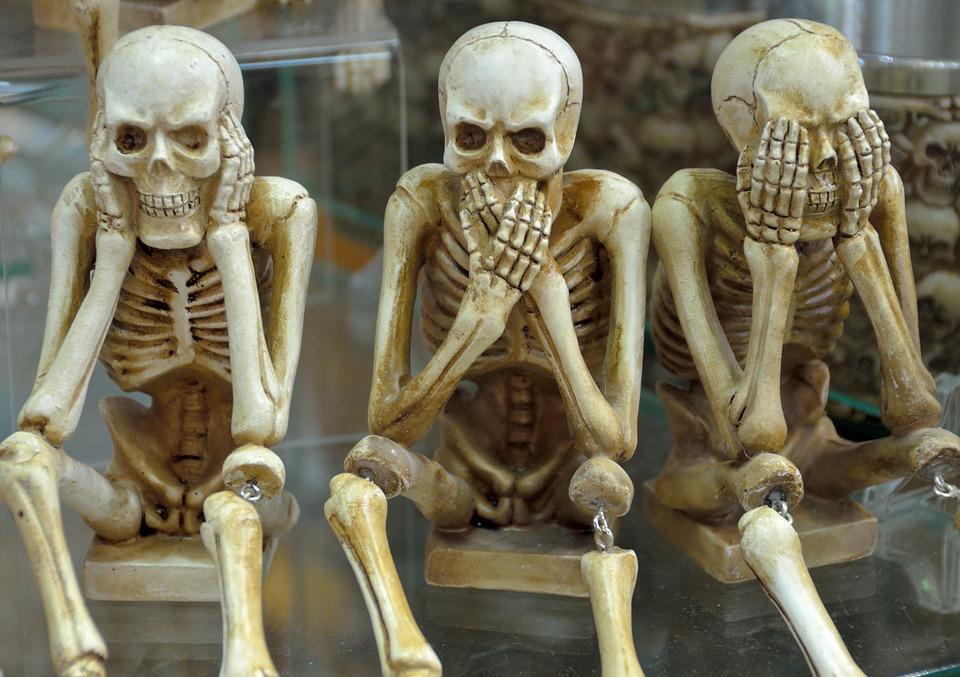
\includegraphics{/home/joe/dev/cpp/CISP440/encryption/cracked.jpg}
\end{document}
